\chapter{Statistical analysis}
To estimate the sensibility of the $tH$ signal, we define an Asimov dataset. Asimov set is a set such that when one uses it to evaluate the estimators for
all parameters, one obtains the true parameter values. This is made by replacing the ensemble of simulated data sets by a single representative one. 
With this Asimov dataset, a fit was applied by using a statistical model built with the signal and backgrounds. In an numerical algorithm is applied a 	minimization for $-\log{(L)}$, where L is the probability from observing the data for the model. Also it is shown  extrapolations of the data for future predictions.

\section{Likelihood and fit procedure}
Suppose for each event in the signal sample one measures a variable x and constructs a histogram $n = (n1, . . . , nN )$ with those measured values. The expectation value of $n_i$ can be written as
$E[ni] = \mu s_i + b_i$ 


The likelihood function is the product of Poisson probabilities for all bins
\begin{align}
L(\mu,\theta)=\prod_{j=1}^{N}\frac{(\mu s_j +b_j)^{n_j}}{n_j !}e^{-(\mu s_j+b_j)}
\end{align}

\begin{itemize}
	\item	N=number of bins
	\item	$\mu$=parameter of signal
	\item	s=signal
	\item	b=background
	\item	n=number of events
\end{itemize}


To test a hypothesized value of $\mu$ we consider the profile likelihood ratio
\begin{align}
\lambda(\mu)=\frac{L(\mu,\hat{\hat{\theta}})}{L(\hat{\mu},\hat{\theta})}
\end{align}

\begin{itemize}
	\item Here $\hat{\hat{\theta}} $ in the numerator denotes the value of $\theta$ that maximizes L for the specified $\mu$,
	it is the conditional maximum-likelihood (ML) estimator of $\hat{\theta}$ (and thus is a function of $\mu$).
	The denominator is the maximized (unconditional) likelihood function, i.e., $\hat{\mu}$ and $\hat{\theta}$ are
	their ML estimators 
	\item The presence of the nuisance parameters broadens the profile likelihood as a
	function of $\mu$ relative to what one would have if their values were fixed. This reflects the loss
	of information about $\mu$ due to the systematic uncertainties
\end{itemize}

For purposes of establishing an upper limit on the strength parameter $\mu$ , we consider two
closely related test statistics. First, we may define
\begin{align} 
q_{\mu}=  \Big\{    \begin{array}{ll}
-2\ln\lambda(\mu) \qquad \hat{\mu} \leq \mu	\\
0  \qquad \qquad \qquad \hat{\mu}< 0 
\end{array}
\end{align}
The reason for setting $q_\mu = 0$
for $\hat{\mu}>\mu $ is that when setting an upper limit, one would not regard data with $\hat{\mu}>\mu $ as
representing less compatibility with $\mu$ than the data obtained, and therefore this is not taken
as part of the rejection region of the test. From the definition of the test statistic one sees that
higher values of $q_\mu$ represent greater incompatibility between the data and the hypothesized
value of $\mu$.







\begin{table}
	\caption{Prefit and postfit table for each yield.Prefit uncertainty is statistical only. Postfit uncertainty is statistical + systematic.}
\begin{tabular}{ccc}
	\hline
	Process  & Number of events prefit    & Number of events Postfit \\
	\hline
$t\bar{t}W$  &  68 $\pm$ 10 & 68$\pm$8.94385\\
	$t\bar{t}Z$  & 25.9 $\pm$ 3.9 & 25.9$\pm$3.839\\
$WZ$ & 15.1$\pm$7.7 & 15.1$\pm$7.49851\\
Rares & 20.9 $\pm$   4.9& 20.86$\pm$4.80068\\
	Fakes  & 80.9 $\pm$9.4  & 80.9$\pm$9.05762\\
$t\bar{t}H$  &  24.2 $\pm$ 2.1 & 24.2$\pm$2.07614\\
\hline
$tH$ & 2.14 $\pm$ 0.13  & 2.14$\pm$16.3986
\end{tabular}	
\end{table}


\begin{figure}
	\centering
	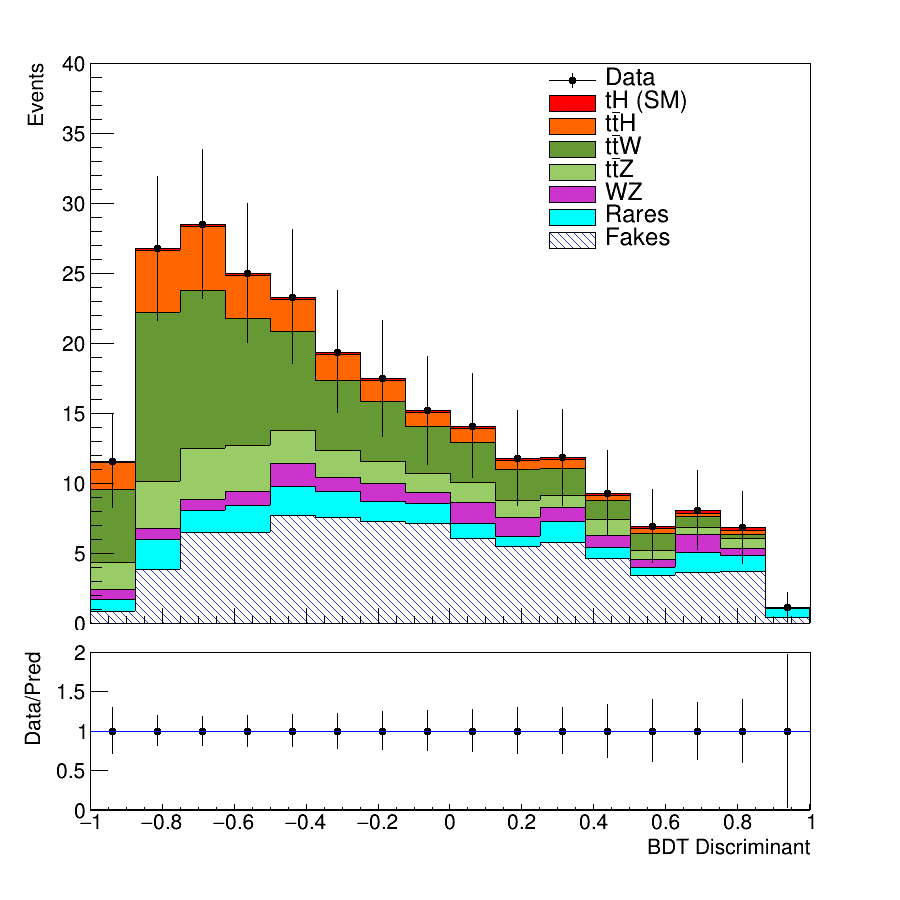
\includegraphics[width=11cm,height=11cm]{Chapter4/kin.png}
	\caption{Pre-fit signal and background yields for tH process for $k_t$=-1.\\
		In the box below each distribution, the ratio of the observed and predicted event yields is shown}
\end{figure}

\begin{table}
	\centering
	Prefit and postfit table for each yield  for . $k_{t}$ =-1..
	\begin{tabular}{|c|c|c|}
		\hline
		Process  & Number of events prefit    & Number of events Postfit\\
		\hline
		tH & 26.2 & 1.83 $\pm$ 26.63\\
		\hline
		t$\bar{t}$H  & 24.18 $\pm$ 2.26& 24.82 $\pm$ 2.27\\
		\hline
		t$\bar{t}$W  & 68.03  $\pm$ 9.54 & 77.07 $\pm$ 8.99\\
		\hline
		t$\bar{t}$Z  & 25.89  $\pm$  3.20& 26.76 $\pm$ 3.18\\
		\hline
		Rares SM & 17.17  $\pm$ 8.64 & 18.90 $\pm$ 8.37\\
		\hline
		WZ & 16.23  $\pm$ 8.17& 17.54 $\pm$ 8.15\\
		\hline
		Non prompt lepton & 80.94   $\pm$ 40.86& 102.97 $\pm$ 29.51\\
		\hline
	\end{tabular}
\end{table}


\begin{figure}
	\centering
	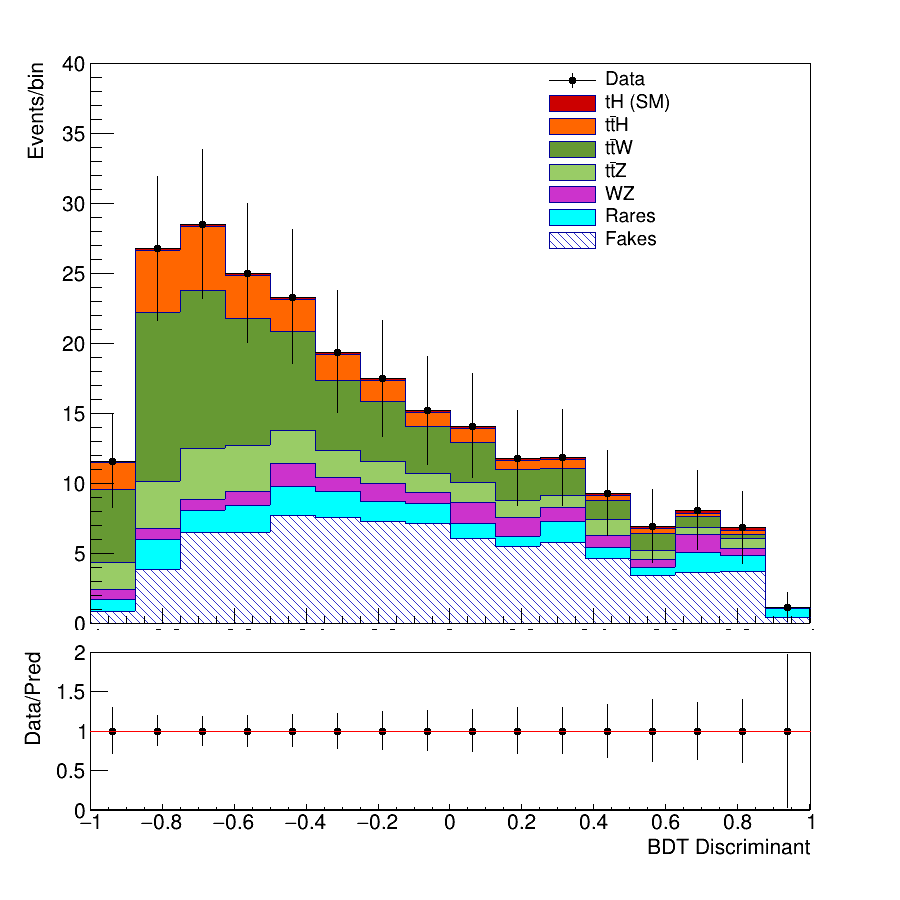
\includegraphics[width=11cm,height=11cm]{Chapter4/simple.png}
	\caption{Post fit signal and background yields for tH process for $k_t$=-1.
		In the box below each distribution, the ratio of the observed and predicted event yields is shown}
\end{figure}




Prefit uncertainty is statistical only. Postfit uncertainty is statistical + systematic.


\begin{figure}
	\centering
	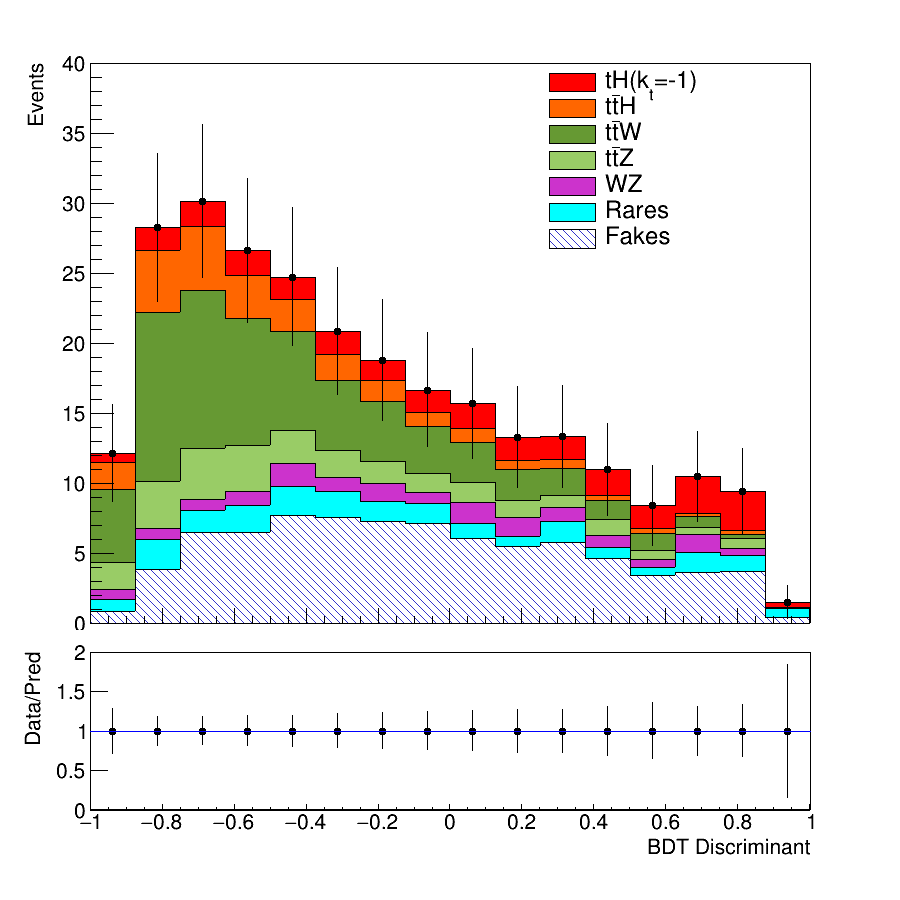
\includegraphics[width=11cm,height=11cm]{Chapter4/kin-kt-1.png}
	\caption{Pre-fit signal and background yields for tH process for $k_t$=-1.\\
		In the box below each distribution, the ratio of the observed and predicted event yields is shown}
\end{figure}



\begin{figure}
	\centering
	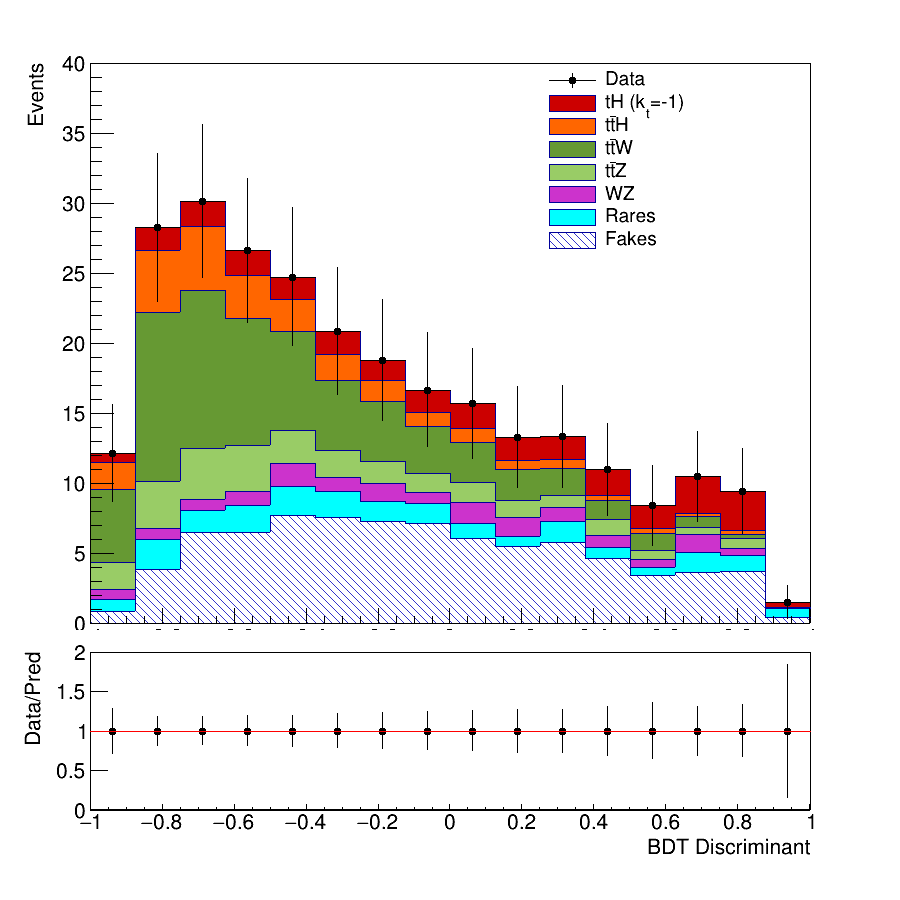
\includegraphics[width=11cm,height=11cm]{Chapter4/simple-kt-1.png}
	\caption{Post fit signal and background yields for tH process for $k_t$=-1.
		In the box below each distribution, the ratio of the observed and predicted event yields is shown}
\end{figure}

\section{Limit calculation}


\begin{table}[ht!]
	\caption{Estimation of $\mu$ and upper limits  for extrapolations}
	\begin{tabular}{|c|c|c|c|c|}
		\hline
		Luminosity (fb$^{-1}$)	&$\mu$ &$\mu$ for $k_t=-1$ &$\mu$ upper limit &$\mu$ upper limit for $k_t=-1$ \\
		\hline
		35.9 & 1.00 $\pm$  8.32 & 1.00 $\pm$  0.249&	22.328 & 2.777   \\
		\hline
		150& 1.00 $\pm$  6.44 & 1.00 $\pm$  0.544  &12.619 &0.915 \\
		\hline
		300&1.00 $\pm$  4.83 &1.00 $\pm$  0.407 & 9.427&0.649 \\
		\hline
		3000&1.00 $\pm$  1.54 & 1.00 $\pm$  0.151&	 3.442 & 0.25
		\\
		\hline
	\end{tabular}
\end{table}

\section{title}